\documentclass{standalone}
\usepackage{tikz}
\usetikzlibrary{patterns, positioning}
\usepackage[sfdefault]{ClearSans} %% option 'sfdefault' activates Clear Sans as the default text font
\usepackage[T1]{fontenc}

\begin{document}
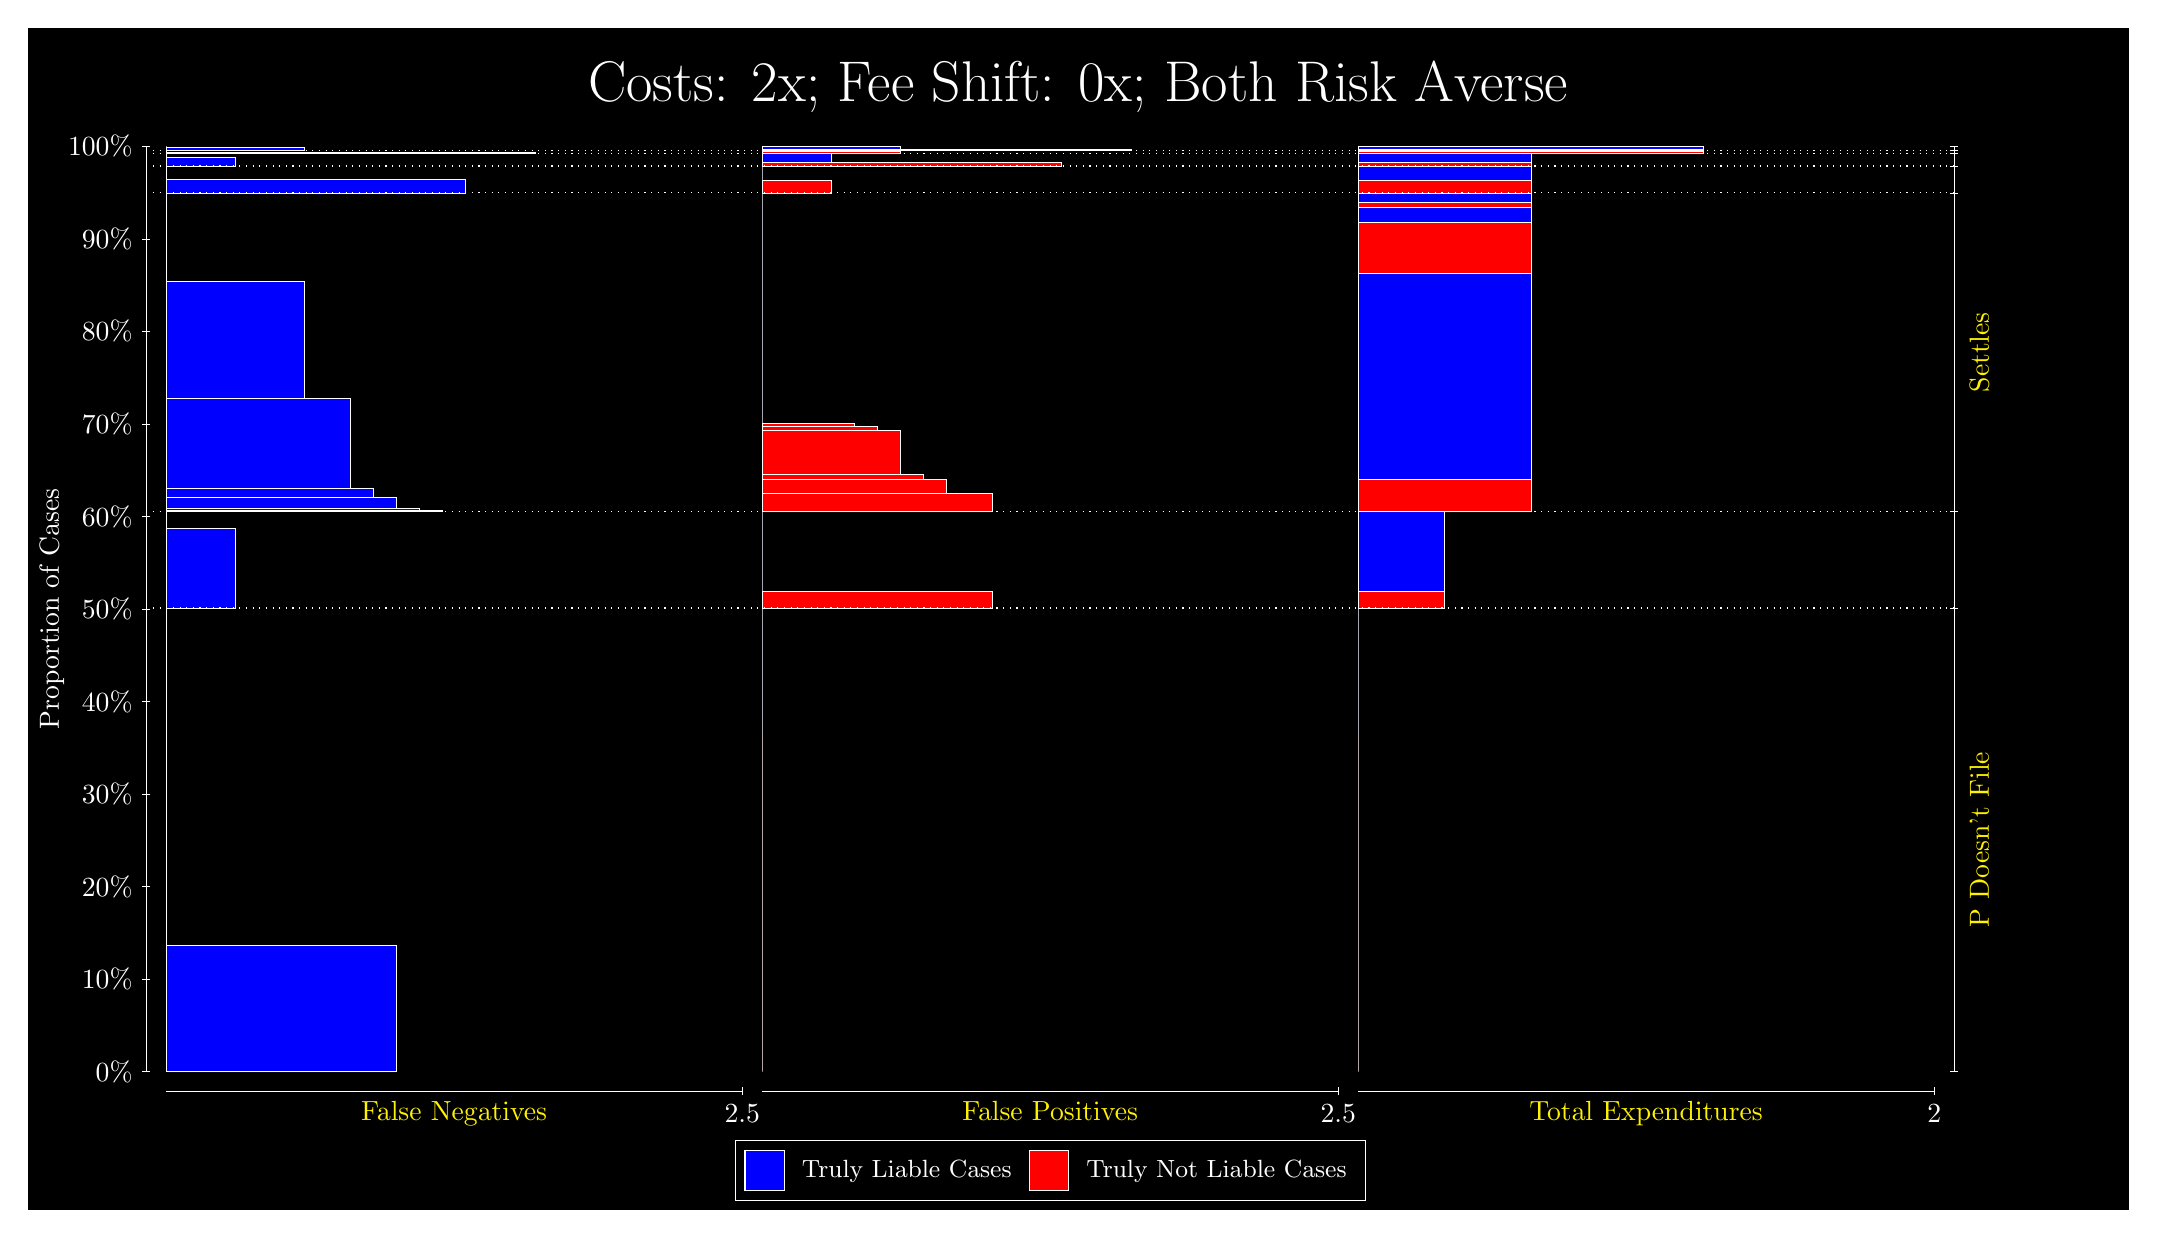
\begin{tikzpicture}
\draw[fill=black] (0,0) rectangle (26.667,15);
\draw[text=white] (0,13.5) rectangle (26.667,15) node[midway] {\huge Costs: 2x; Fee Shift: 0x; Both Risk Averse};
\draw[white, very thin] (1.5,1.75) -- (1.5,13.5);
\node[rotate=90, text=white, anchor=center] at (0.3, 7.625) {Proportion of Cases};
\draw[white, very thin] (1.45,1.75) -- (1.55,1.75);
\node[text=white, anchor=east] at (1.45, 1.75) {0\%};
\draw[white, very thin] (1.45,2.925) -- (1.55,2.925);
\node[text=white, anchor=east] at (1.45, 2.925) {10\%};
\draw[white, very thin] (1.45,4.1) -- (1.55,4.1);
\node[text=white, anchor=east] at (1.45, 4.1) {20\%};
\draw[white, very thin] (1.45,5.275) -- (1.55,5.275);
\node[text=white, anchor=east] at (1.45, 5.275) {30\%};
\draw[white, very thin] (1.45,6.45) -- (1.55,6.45);
\node[text=white, anchor=east] at (1.45, 6.45) {40\%};
\draw[white, very thin] (1.45,7.625) -- (1.55,7.625);
\node[text=white, anchor=east] at (1.45, 7.625) {50\%};
\draw[white, very thin] (1.45,8.8) -- (1.55,8.8);
\node[text=white, anchor=east] at (1.45, 8.8) {60\%};
\draw[white, very thin] (1.45,9.975) -- (1.55,9.975);
\node[text=white, anchor=east] at (1.45, 9.975) {70\%};
\draw[white, very thin] (1.45,11.15) -- (1.55,11.15);
\node[text=white, anchor=east] at (1.45, 11.15) {80\%};
\draw[white, very thin] (1.45,12.325) -- (1.55,12.325);
\node[text=white, anchor=east] at (1.45, 12.325) {90\%};
\draw[white, very thin] (1.45,13.5) -- (1.55,13.5);
\node[text=white, anchor=east] at (1.45, 13.5) {100\%};

\draw[white, very thin] (24.457,1.75) -- (24.457,13.5);
\draw[white, very thin] (24.407,1.75) -- (24.507,1.75);
\node[anchor=west] at (24.407, 1.75) {};
\draw[white, very thin] (24.407,7.6364) -- (24.507,7.6364);
\node[anchor=west] at (24.407, 7.6364) {};
\draw[white, very thin] (24.407,8.8604) -- (24.507,8.8604);
\node[anchor=west] at (24.407, 8.8604) {};
\draw[white, very thin] (24.407,12.908) -- (24.507,12.908);
\node[anchor=west] at (24.407, 12.908) {};
\draw[white, very thin] (24.407,13.25) -- (24.507,13.25);
\node[anchor=west] at (24.407, 13.25) {};
\draw[white, very thin] (24.407,13.414) -- (24.507,13.414);
\node[anchor=west] at (24.407, 13.414) {};
\draw[white, very thin] (24.407,13.445) -- (24.507,13.445);
\node[anchor=west] at (24.407, 13.445) {};
\draw[white, very thin] (24.407,13.5) -- (24.507,13.5);
\node[anchor=west] at (24.407, 13.5) {};

\draw[white, very thin, fill=blue] (1.75,1.75) rectangle (4.6775,3.35);
\draw[white, very thin, fill=red] (1.75,3.35) rectangle (1.75,7.6364);
\draw[white, very thin, fill=blue] (1.75,7.6364) rectangle (2.6283,8.6486);
\draw[white, very thin, fill=red] (1.75,8.6486) rectangle (1.75,8.8604);
\draw[white, very thin, fill=blue] (1.75,8.8604) rectangle (5.2631,8.8759);
\draw[white, very thin, fill=blue] (1.75,8.8759) rectangle (4.9703,8.9077);
\draw[white, very thin, fill=blue] (1.75,8.9077) rectangle (4.6775,9.043);
\draw[white, very thin, fill=blue] (1.75,9.043) rectangle (4.3848,9.1563);
\draw[white, very thin, fill=blue] (1.75,9.1563) rectangle (4.092,10.295);
\draw[white, very thin, fill=blue] (1.75,10.295) rectangle (3.5065,11.781);
\draw[white, very thin, fill=red] (1.75,11.781) rectangle (1.75,12.908);
\draw[white, very thin, fill=blue] (1.75,12.908) rectangle (5.5558,13.084);
\draw[white, very thin, fill=red] (1.75,13.084) rectangle (1.75,13.25);
\draw[white, very thin, fill=blue] (1.75,13.25) rectangle (2.6283,13.361);
\draw[white, very thin, fill=red] (1.75,13.361) rectangle (1.75,13.414);
\draw[white, very thin, fill=blue] (1.75,13.414) rectangle (6.4341,13.427);
\draw[white, very thin, fill=red] (1.75,13.427) rectangle (1.75,13.445);
\draw[white, very thin, fill=blue] (1.75,13.445) rectangle (3.5065,13.487);
\draw[white, very thin, fill=red] (1.75,13.487) rectangle (1.75,13.5);
\draw[white, very thin, fill=red] (9.3189,1.75) rectangle (9.3189,6.0364);
\draw[white, very thin, fill=blue] (9.3189,6.0364) rectangle (9.3189,7.6364);
\draw[white, very thin, fill=red] (9.3189,7.6364) rectangle (12.246,7.8482);
\draw[white, very thin, fill=blue] (9.3189,7.8482) rectangle (9.3189,8.8604);
\draw[white, very thin, fill=red] (9.3189,8.8604) rectangle (12.246,9.0914);
\draw[white, very thin, fill=red] (9.3189,9.0914) rectangle (11.661,9.2654);
\draw[white, very thin, fill=red] (9.3189,9.2654) rectangle (11.368,9.3363);
\draw[white, very thin, fill=red] (9.3189,9.3363) rectangle (11.075,9.8886);
\draw[white, very thin, fill=red] (9.3189,9.8886) rectangle (10.783,9.946);
\draw[white, very thin, fill=red] (9.3189,9.946) rectangle (10.49,9.9874);
\draw[white, very thin, fill=blue] (9.3189,9.9874) rectangle (9.3189,12.908);
\draw[white, very thin, fill=red] (9.3189,12.908) rectangle (10.197,13.073);
\draw[white, very thin, fill=blue] (9.3189,13.073) rectangle (9.3189,13.25);
\draw[white, very thin, fill=red] (9.3189,13.25) rectangle (13.125,13.303);
\draw[white, very thin, fill=blue] (9.3189,13.303) rectangle (10.197,13.414);
\draw[white, very thin, fill=red] (9.3189,13.414) rectangle (11.075,13.432);
\draw[white, very thin, fill=blue] (9.3189,13.432) rectangle (9.3189,13.445);
\draw[white, very thin, fill=red] (9.3189,13.445) rectangle (14.003,13.458);
\draw[white, very thin, fill=blue] (9.3189,13.458) rectangle (11.075,13.5);
\draw[white, very thin, fill=red] (16.888,1.75) rectangle (16.888,6.0364);
\draw[white, very thin, fill=blue] (16.888,6.0364) rectangle (16.888,7.6364);
\draw[white, very thin, fill=red] (16.888,7.6364) rectangle (17.986,7.8482);
\draw[white, very thin, fill=blue] (16.888,7.8482) rectangle (17.986,8.8604);
\draw[white, very thin, fill=red] (16.888,8.8604) rectangle (19.083,9.2654);
\draw[white, very thin, fill=blue] (16.888,9.2654) rectangle (19.083,11.89);
\draw[white, very thin, fill=red] (16.888,11.89) rectangle (19.083,12.541);
\draw[white, very thin, fill=blue] (16.888,12.541) rectangle (19.083,12.724);
\draw[white, very thin, fill=red] (16.888,12.724) rectangle (19.083,12.794);
\draw[white, very thin, fill=blue] (16.888,12.794) rectangle (19.083,12.908);
\draw[white, very thin, fill=red] (16.888,12.908) rectangle (19.083,13.073);
\draw[white, very thin, fill=blue] (16.888,13.073) rectangle (19.083,13.25);
\draw[white, very thin, fill=red] (16.888,13.25) rectangle (19.083,13.303);
\draw[white, very thin, fill=blue] (16.888,13.303) rectangle (19.083,13.414);
\draw[white, very thin, fill=red] (16.888,13.414) rectangle (21.279,13.432);
\draw[white, very thin, fill=blue] (16.888,13.432) rectangle (21.279,13.445);
\draw[white, very thin, fill=red] (16.888,13.445) rectangle (21.279,13.458);
\draw[white, very thin, fill=blue] (16.888,13.458) rectangle (21.279,13.5);
\draw[white, dotted] (1.5,7.6364) -- (24.457,7.6364);
\draw[white, dotted] (1.5,8.8604) -- (24.457,8.8604);
\draw[white, dotted] (1.5,12.908) -- (24.457,12.908);
\draw[white, dotted] (1.5,13.25) -- (24.457,13.25);
\draw[white, dotted] (1.5,13.414) -- (24.457,13.414);
\draw[white, dotted] (1.5,13.445) -- (24.457,13.445);
\draw[white, very thin] (1.75,1.5) -- (9.0689,1.5);
\node[text=yellow, anchor=north] at (5.4094, 1.5) {False Negatives};
\draw[white, very thin] (9.0689,1.45) -- (9.0689,1.55);
\node[text=white, anchor=north] at (9.0689, 1.45) {2.5};

\draw[white, very thin] (9.3189,1.5) -- (16.638,1.5);
\node[text=yellow, anchor=north] at (12.978, 1.5) {False Positives};
\draw[white, very thin] (16.638,1.45) -- (16.638,1.55);
\node[text=white, anchor=north] at (16.638, 1.45) {2.5};

\draw[white, very thin] (16.888,1.5) -- (24.207,1.5);
\node[text=yellow, anchor=north] at (20.547, 1.5) {Total Expenditures};
\draw[white, very thin] (24.207,1.45) -- (24.207,1.55);
\node[text=white, anchor=north] at (24.207, 1.45) {2};

\node[text=yellow, centered, rotate=90] at (24.777, 4.6932) {P Doesn't File};

\node[text=yellow, centered, rotate=90] at (24.777, 10.884) {Settles};





\draw (12.978300999999998,1.5) node[draw=none] (baseCoordinate) {};
\begin{scope}[align=center]
        \matrix[scale=0.5, draw=white, below=0.5cm of baseCoordinate, nodes={draw}, column sep=0.1cm]{
            \node[rectangle, draw, minimum width=0.5cm, minimum height=0.5cm, fill=blue] {}; &
            \node[draw=none, font=\small, text=white] (B) {Truly Liable Cases}; &
            \node[rectangle, draw, minimum width=0.5cm, minimum height=0.5cm, fill=red] {}; &
            \node[draw=none, font=\small, text=white] (B) {Truly Not Liable Cases}; \\
            };
\end{scope}

\end{tikzpicture}
\end{document}